\chapter{Additional Results}
\label{app:additional-results}

This appendix contains companion approximation figures and compact
supporting comparisons. The four-rule comparisons use 100,000 evaluation
pairs per setting. The earlier jackknife investigation is identified
separately below. Complete four-rule rates, validity denominators,
component moments and paired contrasts are supplied in the experiment
supplement.

\section{Companion approximation comparisons}

Figures~\ref{fig:redesign-moments-uniform} and
\ref{fig:redesign-moments-same} repeat the component decomposition for
uniform and same-skew margins at common MI 0.02 nats. All ratios use
the definitions in Chapter~\ref{chap:design}. Identical population tables
under these nulls cancel expected difference bias, while estimation
error in each component remains.

\begin{figure}[!htbp]
\centering
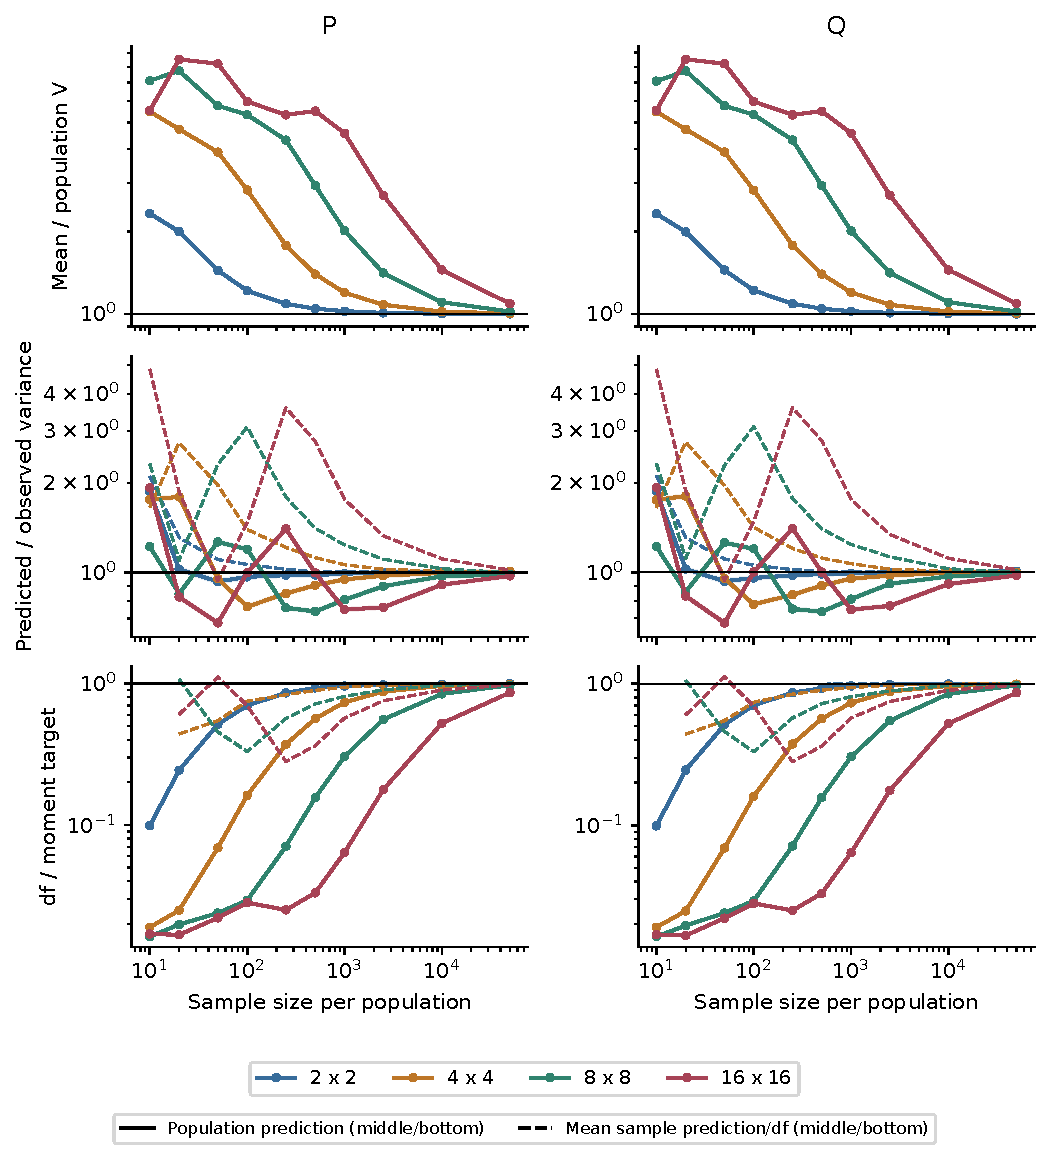
\includegraphics[width=\textwidth,height=.78\textheight,keepaspectratio]{focused_redesign_moments_uniform.pdf}
\caption{Component approximation ratios under uniform margins.}
\label{fig:redesign-moments-uniform}
\end{figure}

\begin{figure}[!htbp]
\centering
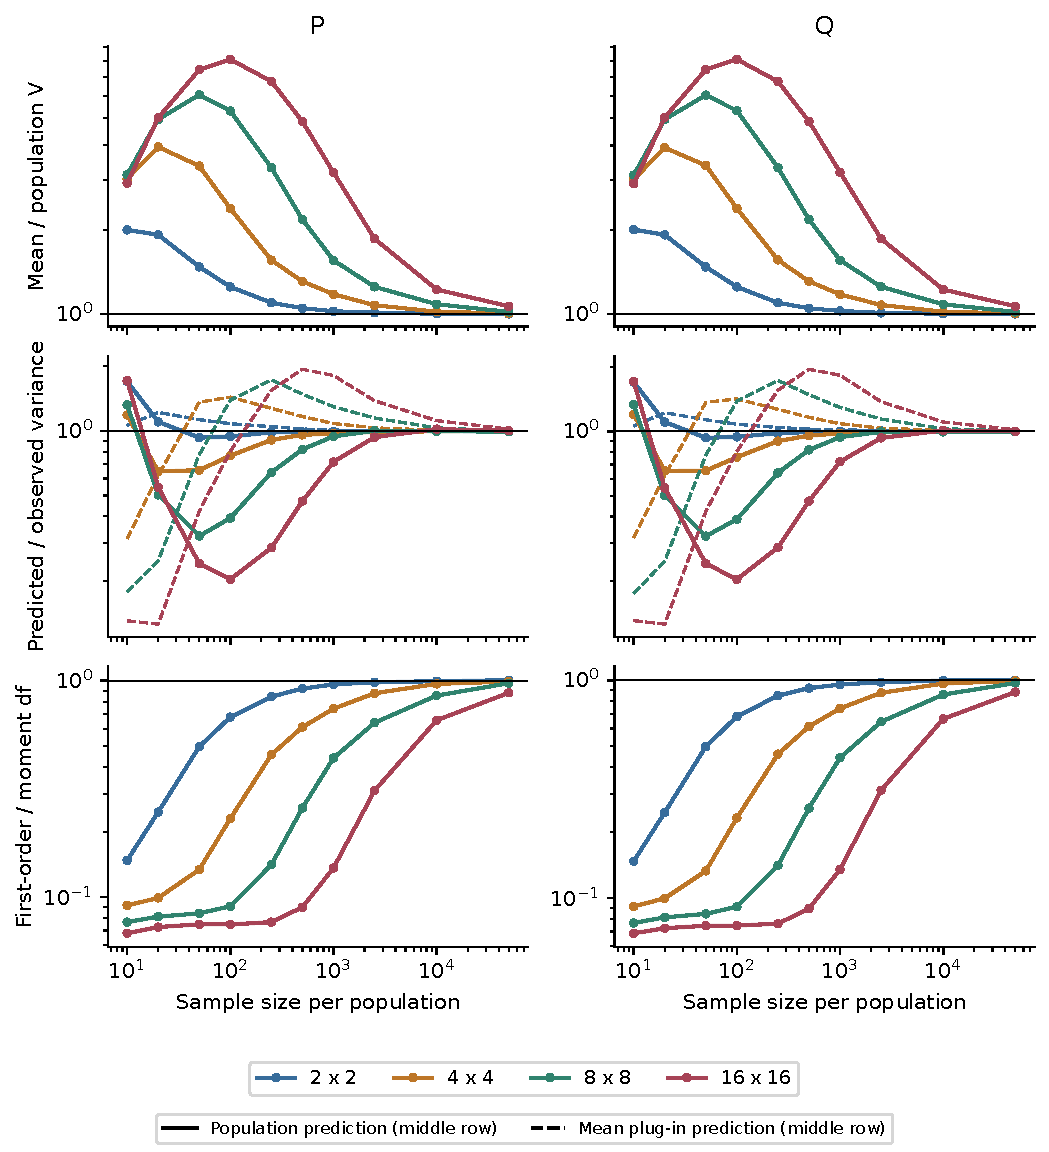
\includegraphics[width=\textwidth,height=.78\textheight,keepaspectratio]{focused_redesign_moments_same_skew.pdf}
\caption{Component approximation ratios under same-skew margins.}
\label{fig:redesign-moments-same}
\end{figure}

Figures~\ref{fig:redesign-a4-small} and \ref{fig:redesign-a4-large}
compare the Appendix A.4 predictions at smaller and larger sample sizes
for the unchanged different-skew MI sweep. Shading gives the fifth--95th
percentile range of the positive finite estimated component degrees of
freedom. It describes sampling spread, rather than uncertainty in a mean.
The companion uniform and same-skew plots are supplied electronically.

\begin{figure}[!htbp]
\centering
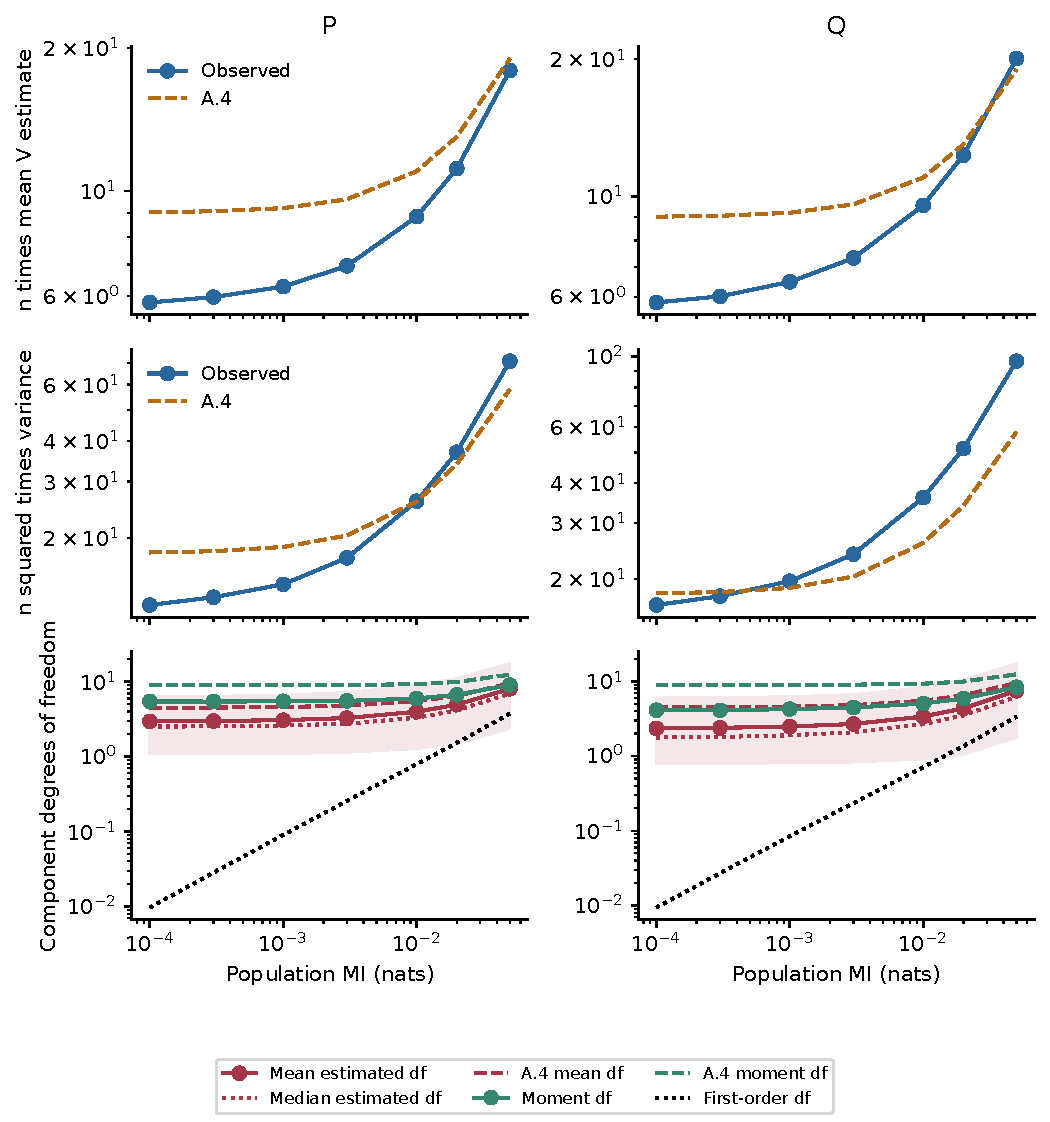
\includegraphics[width=\textwidth,height=.78\textheight,keepaspectratio]{focused_redesign_a4_different_skew_100.pdf}
\caption{Component moments and local predictions at \(n=100\).}
\label{fig:redesign-a4-small}
\end{figure}

\begin{figure}[!htbp]
\centering
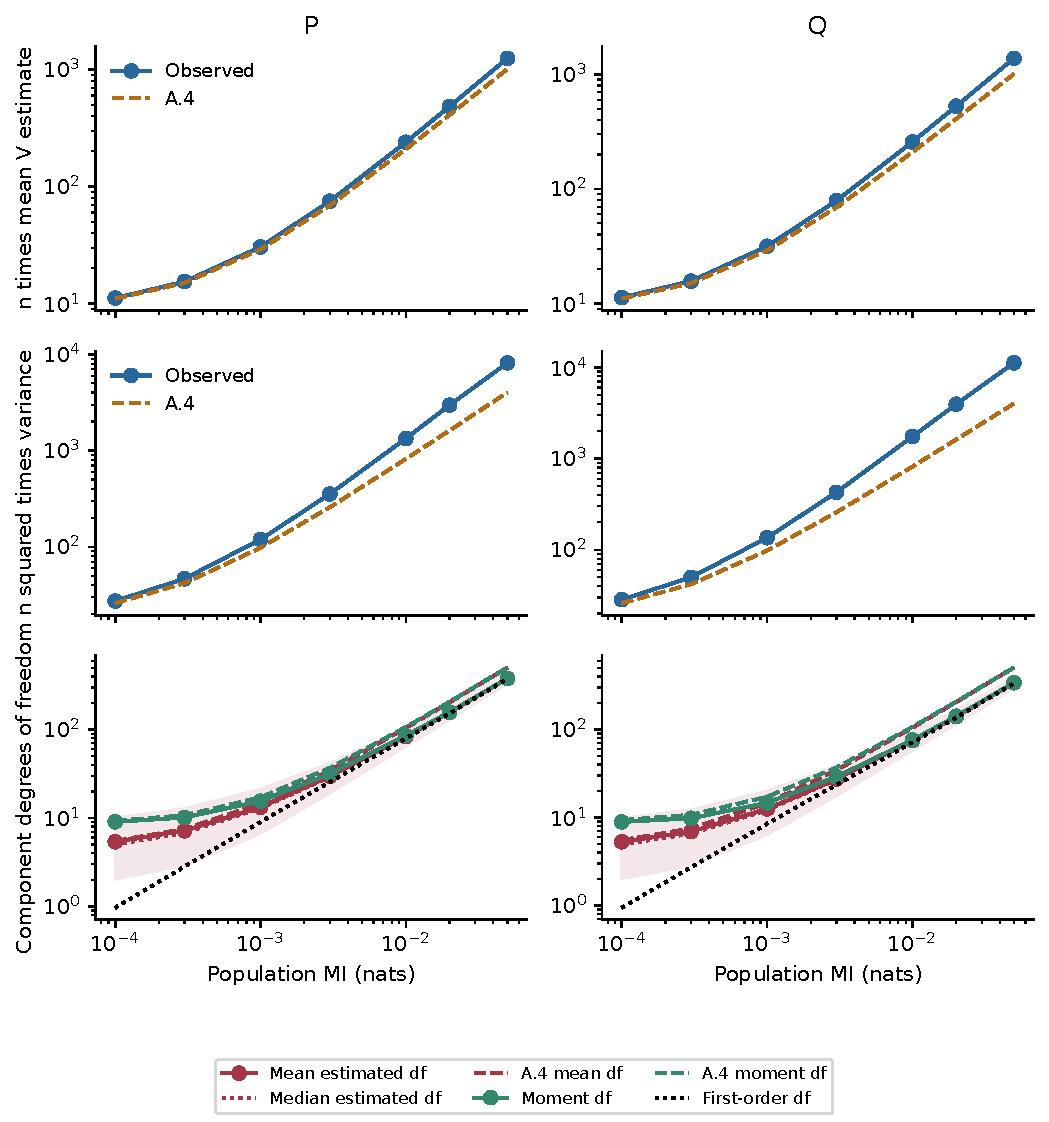
\includegraphics[width=\textwidth,height=.78\textheight,keepaspectratio]{focused_redesign_a4_different_skew_10000.pdf}
\caption{Component moments and local predictions at \(n=10{,}000\).}
\label{fig:redesign-a4-large}
\end{figure}

\section{Component estimates and reference fitting}

Table~\ref{tab:redesign-component-spread} reports the component means,
medians and fifth--95th percentile ranges for the focus and matched
failure settings. The moment target uses the evaluation sampling moments.
All 100,000 component estimates are positive and finite in each shown
row. Their percentile ranges describe variation across samples, not
confidence intervals for a mean. The population-specific summaries
complement the combined values in Chapter~\ref{chap:results}.

\begin{table}[!htbp]
\centering
\small
\setlength{\tabcolsep}{3pt}
\caption{Sampling spread of component degrees of freedom.}
\label{tab:redesign-component-spread}
\begin{tabular}{@{}lrrrrr@{}}
\toprule
Setting, pop. & Mean df & Median df & 5th--95th & Moment df & Included\\
\midrule
A, P & 6.52 & 5.23 & [1.95, 15.32] & 14.81 & 100,000\\
A, Q & 6.54 & 5.24 & [1.93, 15.16] & 14.87 & 100,000\\
B, P & 14.04 & 12.74 & [5.83, 26.60] & 23.54 & 100,000\\
B, Q & 9.72 & 8.47 & [2.64, 20.91] & 12.47 & 100,000\\
C, P & 157.09 & 156.66 & [131.26, 184.27] & 157.96 & 100,000\\
C, Q & 139.70 & 139.28 & [115.88, 165.12] & 141.27 & 100,000\\
16, same, 1,000, P & 39.78 & 39.32 & [29.18, 51.92] & 71.67 & 100,000\\
16, same, 1,000, Q & 39.80 & 39.35 & [29.33, 51.88] & 72.18 & 100,000\\
16, same, 10,000, P & 133.18 & 132.82 & [114.30, 153.25] & 148.48 & 100,000\\
16, same, 10,000, Q & 133.17 & 132.92 & [114.19, 153.21] & 146.84 & 100,000\\
16, different, 1,000, P & 52.58 & 52.08 & [41.98, 64.93] & 87.28 & 100,000\\
16, different, 1,000, Q & 39.80 & 39.33 & [29.15, 51.94] & 71.05 & 100,000\\
16, different, 10,000, P & 172.67 & 172.41 & [152.55, 193.72] & 189.98 & 100,000\\
16, different, 10,000, Q & 133.24 & 132.99 & [114.21, 153.33] & 147.07 & 100,000\\
\bottomrule
\end{tabular}

\end{table}

The fixed references in Table~\ref{tab:redesign-reference-fitting} use
independent 100,000-pair fitting batches. Their Monte Carlo standard
errors follow Appendix~\ref{sec:moment-uncertainty}. The same batches
estimate the null SD used to construct each power path. The constructed
differences are then held fixed, so power uncertainty is conditional on
those population tables. Across all 186 fitting settings, the directly
observed variance of the summed variance contributions differs from the
sum of component variances by at most 0.88\%, consistent with the small
empirical covariances between independently sampled components.

\begin{table}[!htbp]
\centering
\small
\caption{Independent moment references and fitted null standard deviations.}
\label{tab:redesign-reference-fitting}
\begin{tabular}{@{}lrrrr@{}}
\toprule
Setting & Reference df & MCSE & Null SD (nats) & MCSE (nats)\\
\midrule
A & 29.70 & 0.10 & 0.154967 & 0.000363\\
B & 33.34 & 0.11 & 0.065138 & 0.000152\\
C & 293.98 & 0.94 & 0.003175 & 0.000007\\
\bottomrule
\end{tabular}

\end{table}

\section{Same-skew null comparison}

Figure~\ref{fig:redesign-null-same} completes the broad null comparison.
Both populations are identical under the copying construction, so their
expected MI estimation biases cancel at equal sample sizes. Small-sample
conservatism therefore occurs even without an expected difference bias.
The lower panels show validity for Normal Wald and Expanded Welch;
the other two rules share Wald's validity in these settings. Shading
around the rejection curves gives pointwise 95\% Wilson intervals.

\begin{figure}[!htbp]
\centering
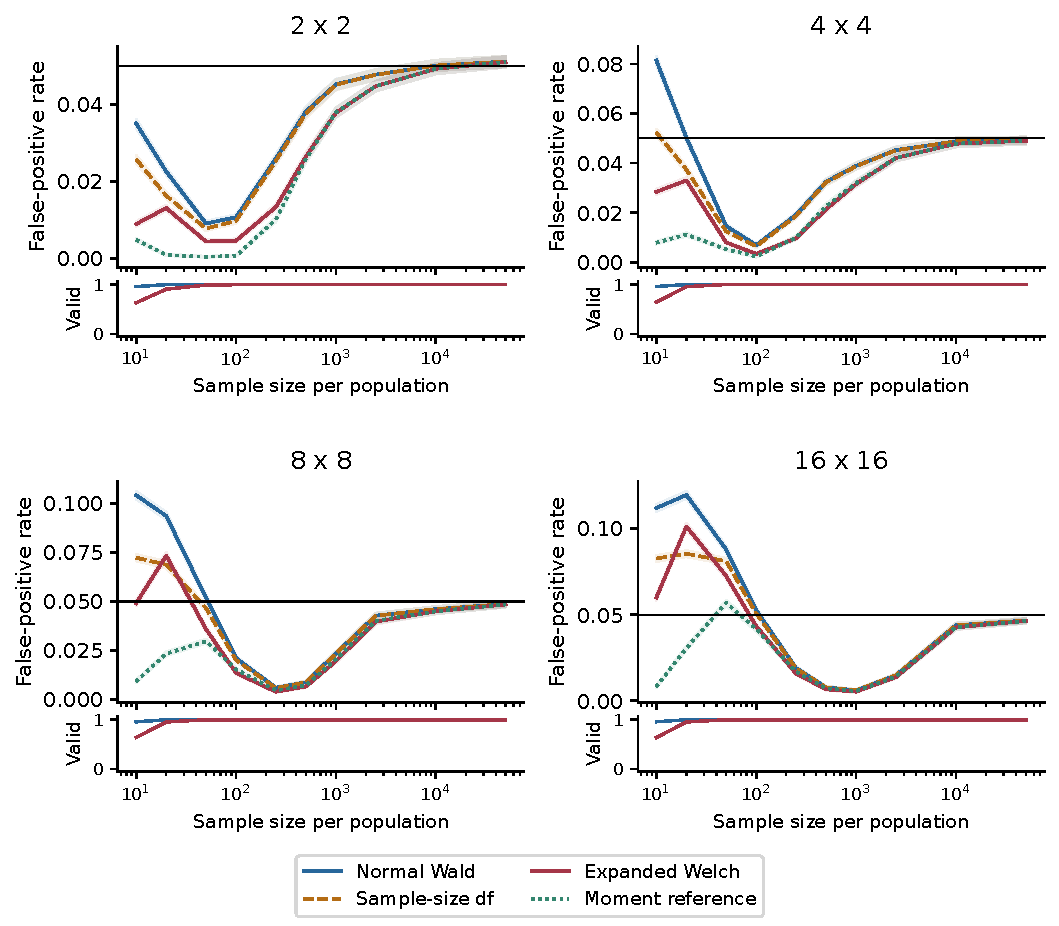
\includegraphics[width=\textwidth]{focused_redesign_null_same_skew.pdf}
\caption{False-positive rates under same-skew margins.}
\label{fig:redesign-null-same}
\end{figure}

\section{Broader power and estimated direction}

Figures~\ref{fig:redesign-broad-different} and
\ref{fig:redesign-broad-same} retain the broader differences in nats at
\(n=1{,}000\) and 10,000. Each curve keeps \(I(P)=0.02\) and increases
\(I(Q)\). They show Normal Wald and Expanded Welch; the complete
four-rule results are in the supplement. Different-skew large tables
show the initial decline associated with the biased estimated difference.
The matched same-skew comparison does not show the same large
wrong-direction rejection problem.

\begin{figure}[!htbp]
\centering
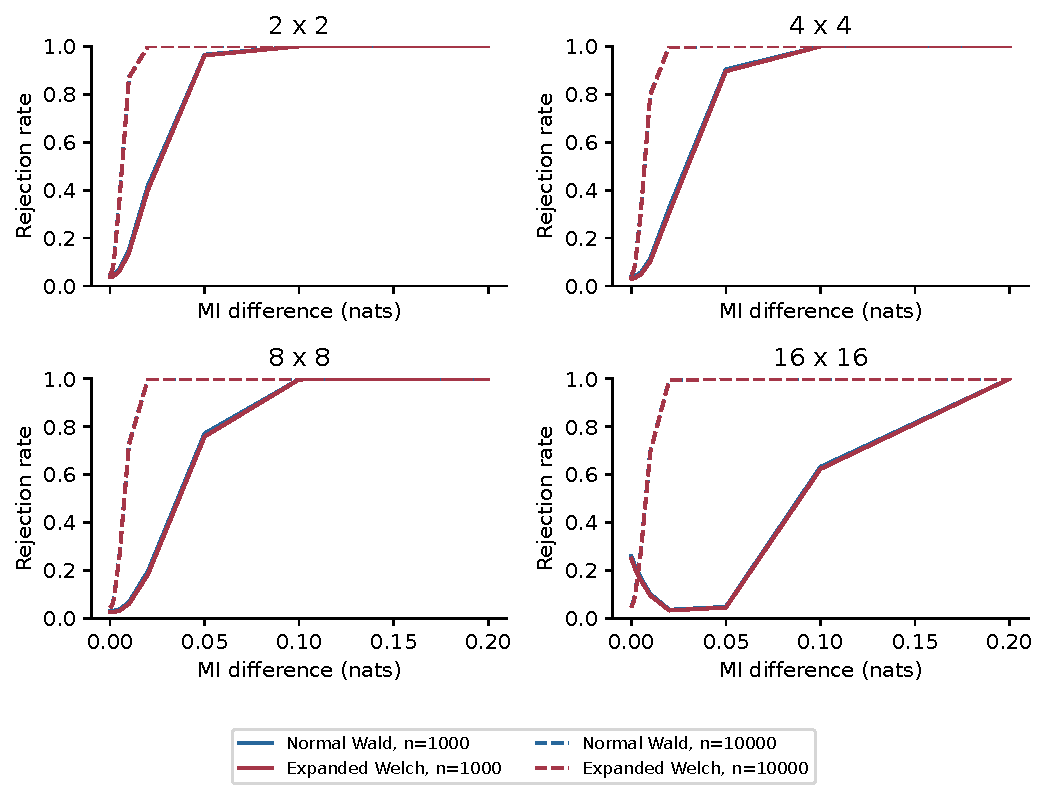
\includegraphics[width=\textwidth]{focused_redesign_broad_power_different_skew.pdf}
\caption{Broader power comparison under different-skew margins.}
\label{fig:redesign-broad-different}
\end{figure}

\begin{figure}[!htbp]
\centering
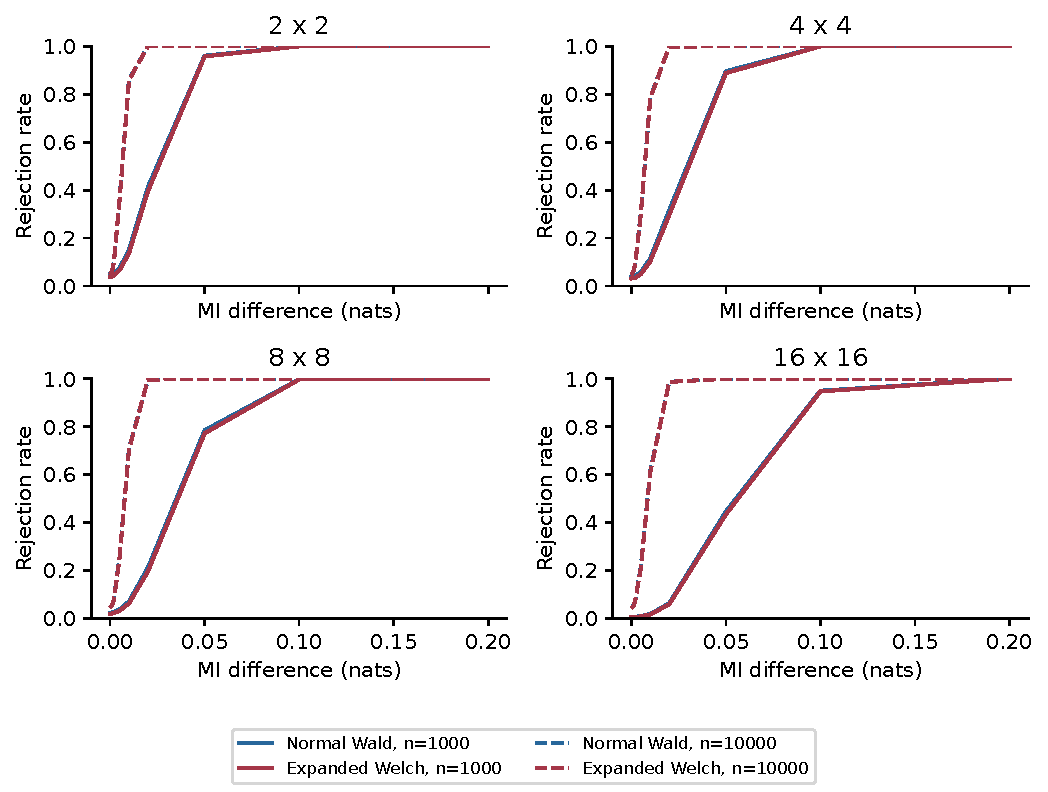
\includegraphics[width=\textwidth]{focused_redesign_broad_power_same_skew.pdf}
\caption{Matched broader power comparison under same-skew margins.}
\label{fig:redesign-broad-same}
\end{figure}

At \(16\times16\), different skew, \(n=1{,}000\) and a true
0.01-nat difference, 10,183 of 10,184 Wald rejections and 9,591 of 9,592
Expanded Welch rejections have the wrong estimated ordering. The fixed
reference gives 9,829 wrong-direction cases among 9,830 rejections.
Under same skew, the corresponding Wald and Expanded Welch counts are
59 of 1,809 and 52 of 1,646. At \(n=10{,}000\), none of the four rules
has a wrong-direction rejection at this alternative under either skew
regime. The different-skew alternative has true difference \(-0.01\) nats, but
its difference bias is 0.03071 nats at \(n=1{,}000\). Thus
\begin{equation}
 \E(\Deltahat)\approx-0.01+0.03071=0.02071\text{ nats}.
 \label{eq:redesign-alternative-bias-shift}
\end{equation}
The positive centre explains why almost every rejection indicates the
wrong ordering. Two-sided power retains every rejection; these counts
show why its interpretation also requires the estimated direction.

\section{Matched construction comparison}

Table~\ref{tab:redesign-construction} compares null rejection under the
copying and four-cell constructions. Each row uses common MI 0.02 nats,
the margin vectors in Chapter~\ref{chap:design}, and equal sample sizes.
The first column identifies table size, skew regime, construction and
sample size. The four-cell construction follows
Equation~\eqref{eq:additive-construction}. Alternative rates and the
corresponding diagnostics are retained in the supplement.

\begin{table}[!htbp]
\centering
\small
\setlength{\tabcolsep}{4pt}
\caption{Matched null rejection under copying and four-cell constructions.}
\label{tab:redesign-construction}
\begin{tabular}{@{}lrrrr@{}}
\toprule
Setting & Wald & Size df & Expanded & Reference\\
\midrule
4, Different, copy, 1000 & 0.0381 & 0.0379 & 0.0316 & 0.0320\\
4, Different, copy, 10000 & 0.0486 & 0.0486 & 0.0477 & 0.0477\\
4, Different, four, 1000 & 0.0387 & 0.0385 & 0.0321 & 0.0322\\
4, Different, four, 10000 & 0.0488 & 0.0487 & 0.0480 & 0.0480\\
4, Same, copy, 1000 & 0.0389 & 0.0387 & 0.0316 & 0.0320\\
4, Same, copy, 10000 & 0.0488 & 0.0488 & 0.0478 & 0.0479\\
4, Same, four, 1000 & 0.0393 & 0.0392 & 0.0325 & 0.0325\\
4, Same, four, 10000 & 0.0491 & 0.0491 & 0.0481 & 0.0480\\
16, Different, copy, 1000 & 0.2601 & 0.2595 & 0.2484 & 0.2535\\
16, Different, copy, 10000 & 0.0478 & 0.0478 & 0.0468 & 0.0469\\
16, Different, four, 1000 & 0.3096 & 0.3090 & 0.2972 & 0.3013\\
16, Different, four, 10000 & 0.0511 & 0.0511 & 0.0501 & 0.0501\\
16, Same, copy, 1000 & 0.0060 & 0.0060 & 0.0053 & 0.0056\\
16, Same, copy, 10000 & 0.0438 & 0.0438 & 0.0426 & 0.0427\\
16, Same, four, 1000 & 0.0113 & 0.0112 & 0.0100 & 0.0104\\
16, Same, four, 10000 & 0.0472 & 0.0471 & 0.0461 & 0.0462\\
\bottomrule
\end{tabular}

\end{table}

\section{Unequal allocation at a fixed total}
\label{sec:allocation-check}

Table~\ref{tab:redesign-allocation} fixes the \(4\times4\) population
pairs and changes the allocation of 2,000 observations. The first column
gives skew regime, \(n_P/n_Q\) and the absolute MI difference in nats.
Null rows use \(I(P)=I(Q)=0.02\), while alternative rows use
\(I(P)=0.02\) and \(I(Q)=0.03\). Each allocation has its own
independently fitted null reference. Reversing the allocation keeps the
population labels and tables fixed.

\begin{table}[!htbp]
\centering
\small
\setlength{\tabcolsep}{4pt}
\caption{Nominal rejection under balanced and unequal allocations.}
\label{tab:redesign-allocation}
\begin{tabular}{@{}lrrrr@{}}
\toprule
Setting & Wald & Size df & Expanded & Reference\\
\midrule
Different, 400/1600, 0.00 & 0.0450 & 0.0446 & 0.0293 & 0.0325\\
Different, 1000/1000, 0.00 & 0.0381 & 0.0379 & 0.0316 & 0.0320\\
Different, 1600/400, 0.00 & 0.0452 & 0.0449 & 0.0251 & 0.0297\\
Different, 400/1600, 0.01 & 0.1324 & 0.1319 & 0.1037 & 0.1070\\
Different, 1000/1000, 0.01 & 0.1148 & 0.1146 & 0.1026 & 0.1018\\
Different, 1600/400, 0.01 & 0.0532 & 0.0523 & 0.0342 & 0.0290\\
Same, 400/1600, 0.00 & 0.0465 & 0.0461 & 0.0270 & 0.0311\\
Same, 1000/1000, 0.00 & 0.0389 & 0.0387 & 0.0316 & 0.0320\\
Same, 1600/400, 0.00 & 0.0462 & 0.0458 & 0.0263 & 0.0310\\
Same, 400/1600, 0.01 & 0.1277 & 0.1273 & 0.0917 & 0.0971\\
Same, 1000/1000, 0.01 & 0.1150 & 0.1147 & 0.1028 & 0.1012\\
Same, 1600/400, 0.01 & 0.0520 & 0.0512 & 0.0349 & 0.0301\\
\bottomrule
\end{tabular}

\end{table}

The allocations change both estimation bias and uncertainty. Even the
same-skew null can retain unequal residual biases when its sample sizes
differ. These comparisons assess the full procedure under imbalance.
The moment identity for combining independent components remains exact;
its accuracy is distinct from the sampling behaviour of the estimated
weights and the distributional approximation for the statistic.

\section{A jackknife check of MI difference bias}
\label{sec:jackknife-difference-check}

This earlier supporting check uses 20,000 pairs per setting, separately
from the 100,000-pair experiment. It asks whether changing the bias
correction improves the sparse
MI differences that give wrong-direction rejections in the main results.
The delete-one jackknife uses the change in an estimate after removing
one observation to estimate its leading finite-sample bias
\citep[Section~3]{paninski2003}.

\begin{samepage}
For the sample from \(P\), let
\(\widehat I^{(-a)}(P)\) be the raw plug-in MI after removing observation
\(a\). Each such estimate uses the remaining \(n_P-1\) observations and
recalculates both margins. Subtracting \(n_P-1\) times the change between
the average leave-one-out estimate and the full-sample estimate gives
\begin{align}
 \widehat I_{\mathrm J}(P)
 &=\Ihat(P)-(n_P-1)
 \left\{\frac{1}{n_P}\sum_{a=1}^{n_P}\widehat I^{(-a)}(P)-\Ihat(P)\right\}
 \notag\\
 &=n_P\Ihat(P)-\frac{n_P-1}{n_P}
 \sum_{a=1}^{n_P}\widehat I^{(-a)}(P).
 \label{eq:jackknife-mi-check}
\end{align}
\end{samepage}
Because observations in the same cell give identical leave-one-out tables,
the average can be calculated once per occupied cell, weighting its
leave-one-out MI by \(N^P_{ij}/n_P\). A cell reduced to zero contributes
zero to the MI sum. Apply the same calculation to \(Q\), retaining
all row and column categories and any negative corrected estimates.

The jackknife replaces the analytic correction in
Equation~\eqref{eq:bias-corrected-difference}. The estimated difference
and statistic become
\begin{equation}
 \widehat\Delta_{\mathrm J}
 =\widehat I_{\mathrm J}(P)-\widehat I_{\mathrm J}(Q),
 \qquad
 T_{\mathrm J}
 =\frac{\widehat\Delta_{\mathrm J}}
 {\sqrt{\Vhat(P)/n_P+\Vhat(Q)/n_Q}}.
 \label{eq:jackknife-fixed-se-check}
\end{equation}
The variance estimates in the denominator are unchanged. Compare
\(|T_{\mathrm J}|\) with the 97.5th percentile of the standard normal
distribution, approximately 1.96, giving the same two-sided 5\% cutoff
as Wald. This separates changing the MI estimate from changing its
estimated uncertainty.

The four settings use \(16\times16\) copying populations with margins
\(m_{16}(0.7)\) for \(P\) and \(m_{16}(0.8)\) for \(Q\), as defined
in Equation~\eqref{eq:skew-margin}. They fix \(I(P)=0.02\) and use
\(I(Q)=0.02\) or 0.03 nats at \(n_P=n_Q=1{,}000\) and 10,000.
Both corrections are applied to the same table pairs in each setting.

\begin{table}[H]
\centering
\small
\caption{Analytic and jackknife MI differences with the same standard error.}
\label{tab:jackknife-difference-check}
\begin{tabular}{@{}rrlrrrr@{}}
\toprule
\(n\) & \(\Delta\) & Correction & Bias & Obs. SD & Est./obs. & \shortstack{Rejection\\rate}\\
\midrule
1,000 & 0.00 & Analytic & +0.02960 & 0.01449 & 1.94 & 0.2522\\
1,000 & 0.00 & Jackknife & -0.00116 & 0.01521 & 1.76 & 0.0085\\
\midrule
1,000 & -0.01 & Analytic & +0.03061 & 0.01564 & 1.81 & 0.1005\\
1,000 & -0.01 & Jackknife & -0.00024 & 0.01638 & 1.65 & 0.0275\\
\midrule
10,000 & 0.00 & Analytic & -0.00088 & 0.00387 & 1.07 & 0.0463\\
10,000 & 0.00 & Jackknife & -0.00045 & 0.00401 & 1.00 & 0.0507\\
\midrule
10,000 & -0.01 & Analytic & -0.00094 & 0.00433 & 1.05 & 0.6992\\
10,000 & -0.01 & Jackknife & -0.00057 & 0.00447 & 0.99 & 0.6619\\
\bottomrule
\end{tabular}

\end{table}

Table~\ref{tab:jackknife-difference-check} shows a much smaller difference
bias at \(n=1{,}000\). Under equal MI, it falls from 0.02960 to
\(-0.00116\) nats; under the alternative, from 0.03061 to
\(-0.00024\) nats. The individual jackknife estimates remain upward
biased. Their null biases are 0.03439 nats for \(P\) and 0.03555 for
\(Q\). Under the alternative, the jackknife MI biases are 0.03452 for
\(P\) and 0.03476 nats for \(Q\).
These similar biases largely cancel in the difference. The observed
standard deviation increases slightly, but the root mean squared error
falls from 0.03295 to 0.01525 nats under the null and from 0.03438 to
0.01638 under the alternative.

The jackknife difference also gives a more accurate estimated ordering at
the sparse alternative. Opposite-direction rejections fall from 2,009 to
5, while correct-direction rejections rise from 1 to 544. The total
rejection rate falls because the original rejections almost all indicate
the wrong ordering. Null rejection, however, falls to 0.0085, with a
Wilson 95\% Monte Carlo interval of [0.0073, 0.0098]. The mean squared
standard error still exceeds the observed variance of the jackknife
difference: their ratio is 1.76 under the null and 1.65 under the
alternative. Better estimation of the difference therefore leaves a
separate problem in estimating its uncertainty.

At \(n=10{,}000\), the jackknife null rejection rate is 0.0507,
with a Wilson interval of [0.0477, 0.0538]. The estimated/observed variance
ratios for the analytic and jackknife differences are both close to one.
Alternative rejection falls from 0.6992 to 0.6619,
with every rejection indicating the correct direction for both
corrections. The jackknife difference has less bias but slightly greater
observed variability and root mean squared error at this sample size.

\section{Computational cost}
\label{sec:timing-procedure}

Table~\ref{tab:focused-runtime} compares scalar-call times, measured separately from sampling and
population construction.
It uses 200 pre-generated different-skew null pairs at \(n=1{,}000\)
for each table size. After 20 warm-up calls per method, five timed passes
through those pairs give 1,000 calls per method and setting. The call
order alternates between passes. Measurements were made on an arm64
machine with macOS 26.6.2, Python 3.13.5, NumPy 2.4.4 and SciPy 1.17.1.
These measurements concern Normal Wald and Expanded Welch;
they do not time the two additional simulation benchmarks.

\begin{table}[!htbp]
\centering
\small
\caption{Time per scalar test call in microseconds: median [interquartile range].}
\label{tab:focused-runtime}
\begin{tabular}{@{}lrr@{}}
\toprule
Size & Normal Wald & Expanded Welch\\
\midrule
\(2\times2\) & 101.83 [99.25, 104.87] & 186.58 [182.46, 191.67]\\
\(4\times4\) & 107.85 [101.92, 113.51] & 197.13 [188.83, 205.25]\\
\(8\times8\) & 103.46 [101.12, 107.30] & 191.81 [187.00, 197.26]\\
\(16\times16\) & 112.42 [108.33, 116.43] & 202.29 [198.07, 208.00]\\
\bottomrule
\end{tabular}

\end{table}

Expanded Welch takes approximately 1.8--1.9 times as long in these
measurements. Both methods require calculations over the table cells,
and the fixed call overhead remains material at these dimensions.

\section{Holm adjustment for the application}
\label{sec:application-holm}

Table~\ref{tab:application-holm} gives the raw and adjusted p-values for
all six comparisons used to select the online-shopping application.
Each tests equal predictor--outcome MI between two groups. Adult compares
female and male records using education (16 categories) or occupation
(14 categories) and income above US\$50,000 \citep{becker1996}. Its
training and test partitions are combined without survey weights;
records with missing occupation are excluded only from that comparison.
Student Performance compares schools GP and MS using Portuguese-language
course records, study time (four levels) or maternal education (five levels),
and a final grade of at least 10 \citep{cortez2008}. The shopping
comparisons use month or weekend and purchasing among new and returning visitors.

\begin{table}[H]
\centering
\small
\caption{Raw and Holm-adjusted p-values for the six exploratory comparisons.}
\label{tab:application-holm}
\setlength{\tabcolsep}{4pt}
\begin{tabularx}{\textwidth}{@{}>{\raggedright\arraybackslash}Xrrrr@{}}
\toprule
& \multicolumn{2}{c}{Normal Wald} & \multicolumn{2}{c}{Expanded Welch}\\
\cmidrule(lr){2-3}\cmidrule(l){4-5}
Comparison & Raw & Adjusted & Raw & Adjusted\\
\midrule
Adult: occupation & \(1.18\times10^{-44}\) & \(7.10\times10^{-44}\) & \(1.64\times10^{-42}\) & \(9.81\times10^{-42}\)\\
Adult: education & \(1.89\times10^{-34}\) & \(9.45\times10^{-34}\) & \(4.93\times10^{-33}\) & \(2.46\times10^{-32}\)\\
Online Shoppers: month & \(4.71\times10^{-5}\) & \(1.89\times10^{-4}\) & \(3.73\times10^{-4}\) & \(1.49\times10^{-3}\)\\
Student Performance: study time & 0.1982 & 0.5946 & 0.2339 & 0.7016\\
Student Performance: maternal education & 0.8361 & 1 & 0.8468 & 1\\
Online Shoppers: weekend & 0.9554 & 1 & 0.9601 & 1\\
\bottomrule
\end{tabularx}
\end{table}

Holm's multiple-testing adjustment is applied separately to each method's
six p-values \citep{holm1979}. Order the raw p-values from smallest to largest and
multiply them by 6, 5, 4, 3, 2 and 1, respectively. Moving through that
order, replace any value smaller than the preceding adjusted value by
that preceding value, and cap the results at one. The month--purchase comparison has the
third-smallest raw p-value for both methods, and the earlier adjusted
values are smaller, so its adjusted p-value is four times its raw value.
Both adjusted month p-values remain below 0.05.
